\documentclass{standalone}
\usepackage{../../../../preamble_tikz}

\begin{document}
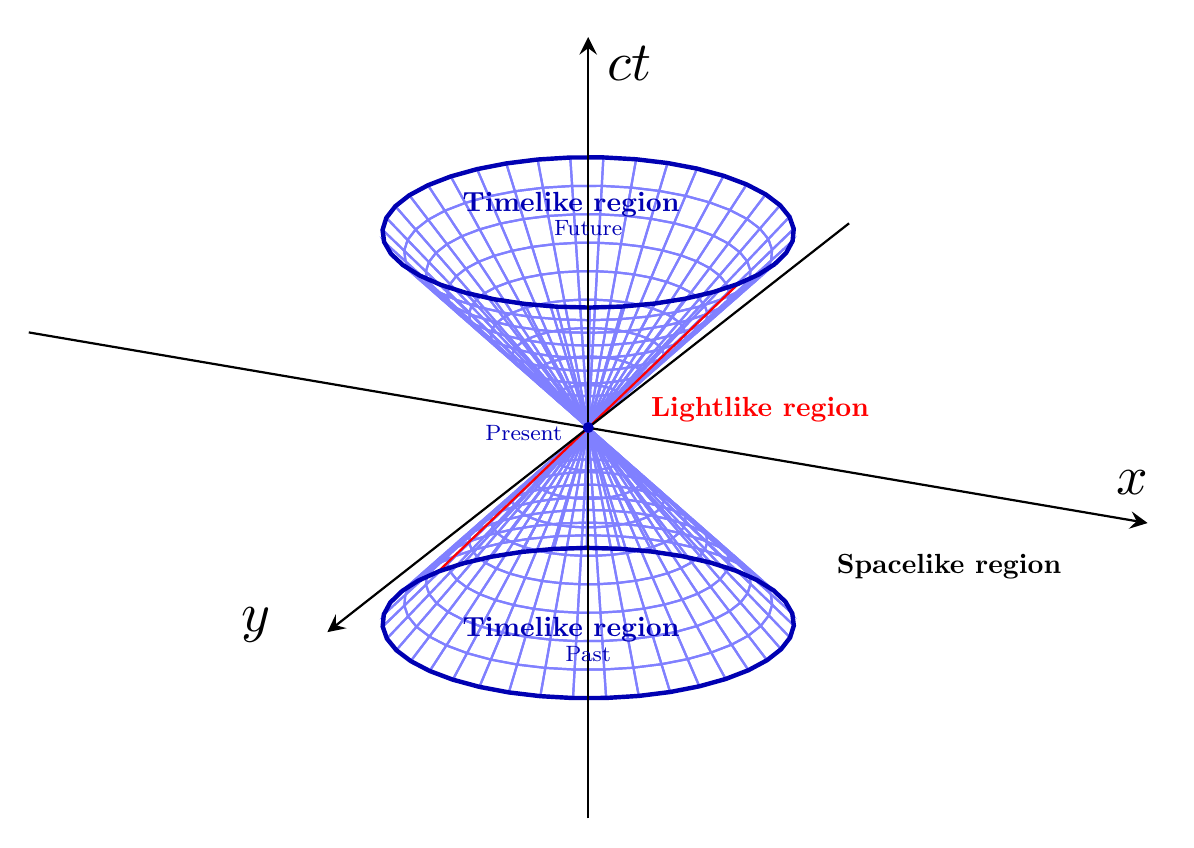
\begin{tikzpicture}[scale=2]
  \begin{axis}[
      width=12cm,
      axis lines=center,
      axis on top,
      xlabel={$x$}, ylabel={$y$}, zlabel={$ct$},
      xtick=\empty, ytick=\empty, ztick=\empty,
      domain=-2:2,
      y domain=0:2*pi,
      xmin=-6, xmax=6,
      ymin=-6, ymax=6,
      zmin=-4, zmax=4,
      samples=10,
      samples y=40,
      y dir=reverse,
      every axis y label/.append style={at=(ticklabel* cs:0)}]
    ]

    % blue cone
    \addplot3 [mesh,draw=blue!50,samples=20] ({x*cos(deg(y))},{x*sin(deg(y))},{x});

    % red line
    \addplot3 [draw=red,samples=10] ({1.5*x},{1.5*x},{1.5*x});

    % blue circles
    \addplot3 [thick,draw=blue!70!black,samples=20] ({2*cos(deg(y))},{2*sin(deg(y))},{2});
    \addplot3 [thick,draw=blue!70!black,samples=20] ({-2*cos(deg(y))},{-2*sin(deg(y))},{-2});
  \end{axis}
  % text
  \node[blue!70!black,font=\bfseries] at (5.1,3.1){Timelike region};
  \node[blue!70!black,font=\bfseries] at (5.1,5.8){Timelike region};
  \node[red,font=\bfseries] at (6.3,4.5,0){Lightlike region};
  \node[font=\bfseries] at (7.5,3.5,0){Spacelike region};

  \node[blue!70!black,font=\footnotesize] at (5.209,2.95){Past};
  \node[blue!70!black,font=\footnotesize] at (4.8,4.35){Present};
  \node[blue!70!black,font=\footnotesize] at (5.209,5.65){Future};


  % black ball
  \node[circle,fill=blue!70!black,inner sep=0pt,minimum height=4pt] (c) at (5.209,4.385,0){};
\end{tikzpicture}
\end{document}
